\documentclass{article}%
\usepackage[T1]{fontenc}%
\usepackage[utf8]{inputenc}%
\usepackage{lmodern}%
\usepackage{textcomp}%
\usepackage{lastpage}%
\usepackage[head=40pt,margin=0.5in,bottom=0.6in]{geometry}%
\usepackage{graphicx}%
%
\title{\textbf{Emiten orden de arresto en EEUU contra el actor Fernando Carrillo}}%
\author{Diario El Universal}%
\date{07/03/2019}%
%
\begin{document}%
\normalsize%
\maketitle%
\textbf{URL: }%
http://www.eluniversal.com/entretenimiento/34987/emiten{-}orden{-}de{-}arresto{-}en{-}eeuu{-}contra{-}el{-}actor{-}fernando{-}carrillo\newline%
%
\textbf{Periodico: }%
EU, %
ID: %
34987, %
Seccion: %
entretenimiento\newline%
%
\textbf{Palabras Claves: }%
NO\_TIENE\newline%
%
\textbf{Derecho: }%
2.1%
, Otros Derechos: %
\newline%
%
\textbf{\textit{El protagonista de "Abigaíl" fue demandado por deber 15.000 dólares de manutención a su hijo}}%
\newline%
\newline%
%
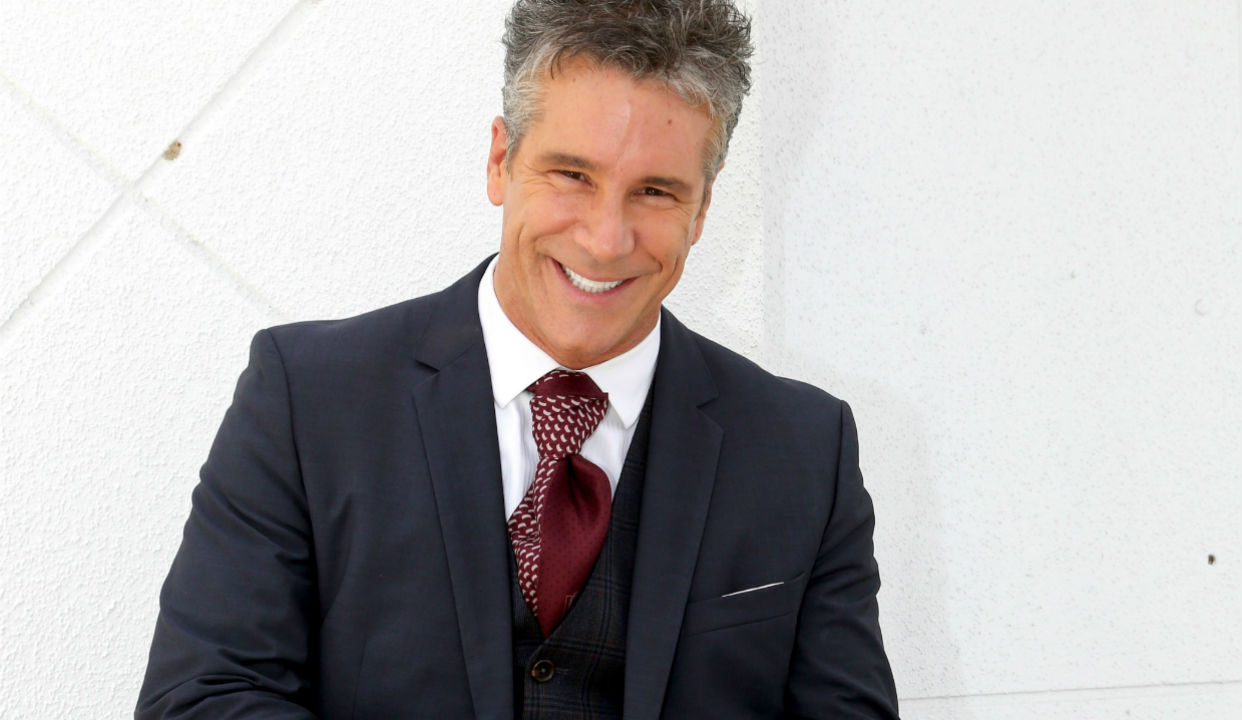
\includegraphics[width=300px]{EU_34987.jpg}%
\newline%
%
Un tribunal de Miami, Florida, dictó una orden de aprehensión contra el actor, modelo y cantante Fernando Carrillo, por el incumplimiento del pago de la pensión alimentaria de su hijo Ángel Gabriel.%
\newline%
%
Según reseñó el portal de noticias~Infobae, la madre del menor, Margiolis Ramos, aseguró que la estrella de televisión debe 15.000 dólares de manutención, y que no ha querido hacerse responsable de los gastos de su hijo desde iniciaran una querella legal hace cuatro años.%
\newline%
%
"En principio él me daba USD 1.200, cuando pusimos la cuestión en la corte, él lo había bajado a USD 600 mientras estaba la decisión de la juez, y él se fue del país y dejó de pagar desde mayo del año pasado", indicó la mujer en el programa de TV Azteca Ventaneando, donde además de no responder a la orden judicial, Carrillo se desentendió por completo del niño, a quien no ve desde hace año y medio.%
\newline%
%
Ramos, quien trabaja como vendedora a través del servicio Uber Eats, señaló que el protagonista de Abigaíl recientemente la invitó a venir a México para llegar a un acuerdo extrajudicial, pero reiteró que no retirará su demanda hasta que se arregle en una corte de Estados Unidos.%
\newline%
%
Por su parte Carrillo, que actualmente vive en México, respondió en el programa Primer Impacto de la cadena Univisión que las acusaciones son totalmente falsas y se ha intentado mediatizar la situación en lo que catalogó como "parte de show, del rock and roll".%
\newline%
%
"Lamentablemente se ha vuelto mediático no porque lo he querido, y es algo que afecta al niño, por eso me mantengo al margen, siempre estoy para él, pero los tiempos de Dios son perfectos, creo que está creciendo con amor y eso me mantiene tranquilo", dijo el actor, quien además sostuvo que sí mantiene contacto telefónico con su hijo.%
\newline%
%
De momento, Carrillo no podrá pisar territorio estadounidense, pues sería inmediatamente detenido por las autoridades.%
\newline%
%
\end{document}